\documentclass{standalone}
\usepackage{tikz}
\usetikzlibrary{positioning, shapes.geometric}
\usepackage{amsfonts}
\usepackage{amsmath}

%\usepackage[scaled]{helvet} % Load Helvetica font
%\renewcommand*\familydefault{\sfdefault} % Set the default font to the sans serif family
%\usepackage[T1]{fontenc}

\begin{document}

    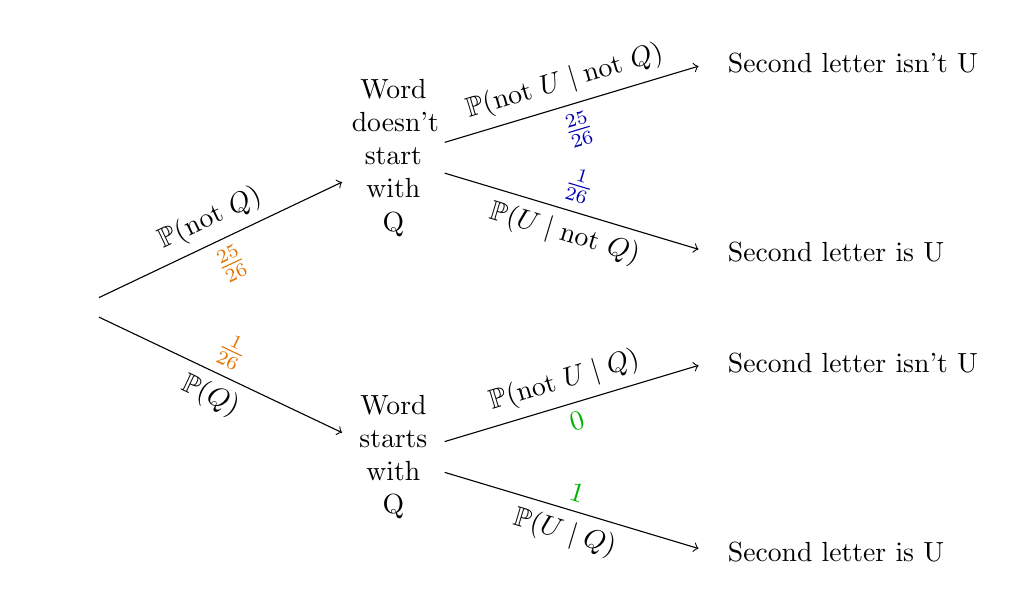
\begin{tikzpicture}[->, grow=right, sloped,
    level 1/.style={sibling distance=3.8cm, level distance=4cm},
    level 2/.style={sibling distance=2.4cm, level distance=4cm},
    level 3/.style={sibling distance=0.6cm,},
    level 4/.style={sibling distance=0.4cm,}]
    \tikzstyle{bag} = [text width=3em, text centered] % Define bag style
    \tikzstyle{end} = [text width=0em, text centered] % Define end style

    \node[bag] {} % Root node with bag style
        child {
            node[bag] {Word starts with Q} % Bag node
                child {
                    node[end, label=right: {Second letter is U}] {} % End node with label
                    edge from parent
                    node[above] {\scalebox{1}{\textcolor{green!70!black}{1}}} % Label above the edge
                    node[below] {$\mathbb{P}(U \mid Q)$} % Label below the edge
                }
                child {
                    node[end, label=right: {Second letter isn't U}] {} % End node with label
                    edge from parent
                    node[above] {$\mathbb{P}(\text{not }U \mid Q)$} % Label above the edge
                    node[below] {\scalebox{1}{\textcolor{green!70!black}{0}}} % Label below the edge
                }
                edge from parent 
                node[above] {\textcolor{orange!90!black}{$\frac{1}{26}$}}
                node[below] {$\mathbb{P}(Q)$} % Label below the edge
        }
        child {
            node[bag] {Word doesn't start with Q} % Bag node
                child {
                    node[end, label=right: {Second letter is U}] {} % End node with label
                    edge from parent
                    node[above] {\scalebox{1}{\textcolor{blue!70!black}{$\frac{1}{26}$}}} % Label above the edge
                    node[below] {$\mathbb{P}(U \mid \text{not }Q)$} % Label below the edge
                }
                child {
                    node[end, label=right: {Second letter isn't U}] {} % End node with label
                    edge from parent
                    node[above] {$\mathbb{P}(\text{not }U \mid \text{not }Q)$} % Label above the edge
                    node[below] {\scalebox{1}{\textcolor{blue!70!black}{$\frac{25}{26}$}}} % Label below the edge
                }
                edge from parent         
                node[above] {$\mathbb{P}(\text{not }Q)$} % Label above the edge
                node[below] {\scalebox{1}{\textcolor{orange!90!black}{$\frac{25}{26}$}}} % Label below the edge
        };
    \end{tikzpicture}

\end{document}
